En este capítulo se detalla cada uno de los puntos llevados a cabo para la realización de este proyecto, empezando por definir la propuesta realizada, luego explicar el proceso ingenieril llevado a cabo y terminar desglosando el trazado de la ejecución de este proyecto.

\section{Propuesta}

El trabajo propuesto tiene como objetivo la creación de un elemento software funcional que, usando el paradigma lógico explicado en la Sección \ref{subsec:asp}, permita la generación de un área que contenga una planificación de un polígono industrial que pueda ser generado y jugado dentro del mapa de \cities. Así mismo incluirá una interfaz gráfica interactuable que permitan al usuario marcar que zonas del terreno deben generarse y cuales no, indicando su contenido antes de lanzar el proceso de generación. \\

Antes de proceder a explicar como se ha llevado a cabo, procederemos a explicar como funciona la industria en \cities.

\subsubsection{Definición de Industria}
\label{subsubsec:terrain}

Una de las principales mecánicas en \cities es la de crear zonas de los diferentes tipos de edificios que se construir en las zonas adyacentes a las carreteras, tal y como se muestra en la Figura \ref{fig:zoneo}. Estas zonas se dividen en una cuadrícula de 5 de ancho a lo largo de la carretera, en donde cada celda es de 8x8 metros. En estas zonas se pueden definir los siguientes tipos descritos a continuación.

\begin{figure}[!h]
	\centering
	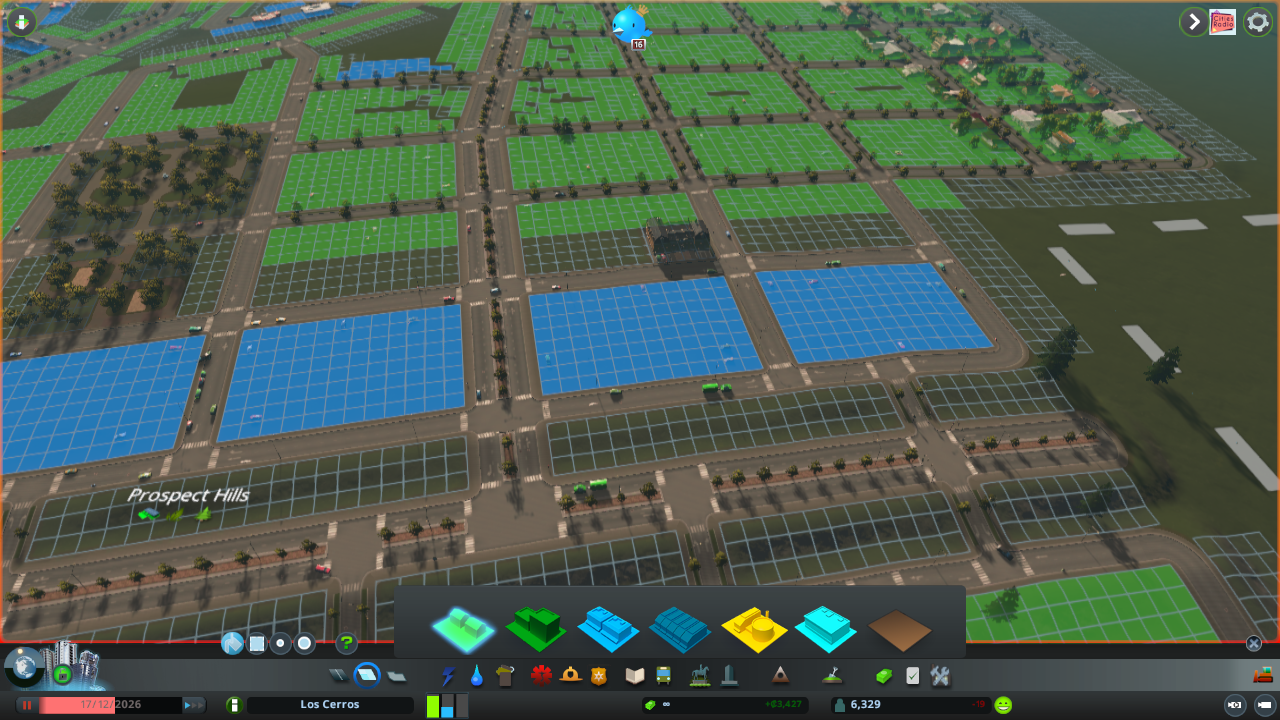
\includegraphics[width=\textwidth]{images/zoneo}
	\caption{Ejemplo de definición de zonas. En la azul las zonas comerciales y en verde las residenciales.}
	\label{fig:zoneo}
\end{figure}

\begin{itemize}
	\item \textbf{Residencial}: Corresponde a las casas donde la gente vivirá.
	\item \textbf{Comercial}: Se refiere a las tiendas y otros servicios que venden los productos creados por la industria o que son exportados.
	\item \textbf{Industrial}: Las zonas industriales proveen trabajo a los ciudadanos y crean los productos de consumo para los edificios comerciales.
	\item \textbf{Oficinas}: Las zonas de oficina dan trabajo solo a ciudadanos con alto nivel de estudios. Además no producen ni contaminación, ni tráfico, ni productos de consumo.
	\item \textbf{Servicios}: En esta categoría entran los edificios que no se pueden crear mediante zonas, si no que se fijan su construcción. Pertenecen al gobierno y dan servicios a los ciudadanos, como parques, cuarteles de policía, estaciones de buses, etc.
\end{itemize}

En este proyecto nos centraremos en las zonas industriales. Son una de las zonas que aumentan el tráfico intensamente, por lo que su planificación debe ser rigurosa. Las zonas industriales se dividen en varios tipos dependiendo de los recursos naturales que puedan usar, que pueden ser renovables (suelo fértil) o no renovables (petroleo y minerales).

\begin{itemize}
	\item \textbf{Genérica}: No tiene una especialización, por lo que corresponde a edificios genéricos. Es una de las más contaminantes pero es la base de la cadena de suministro en \cities. Proveen de trabajos para personas de estudios bajos.
	\item \textbf{Granjas}: Necesitan de suelo fértil (que es renovable) para producir recursos sin producir contaminación. Solo da trabajo para ciudadanos con nivel de estudios bajo.
	\item \textbf{Bosques}: No contamina el suelo pero genera un nivel de ruido significante. Consume también más electricidad que la industria genérica. También da trabajo para gente con nivel de estudios bajo.
	\item \textbf{Petróquímica}: Usa el suelo que contiene petróleo (que no es renovable) para producir combustible. Genera ingresos por impuestos altos, así como altos niveles de polución y consumo alto de energía.
	\item \textbf{Minera}: Usa zonas con minerales (recurso no renovable) para producir carbón. Produce menos polución e ingresos que la petroquímica pero usa más energía que la industria genérica.
\end{itemize}

Desde el lanzamiento de la expansión \textit{Industries}, se agregó un sistema producción, en donde se pueden procesar los recursos naturales hasta obtener productos de consumo de lujo. Para ello existen cinco tipos de edificios: extractores, procesadores, factorías, auxiliares y almacenes. Los edificios auxiliares dan zonas para que los trabajadores vivan y ofrecen mantenimiento, mientras que los almacenes sirven para guardar cada uno de los productos de cada una de las etapas.

\begin{figure}[!h]
	\centering
	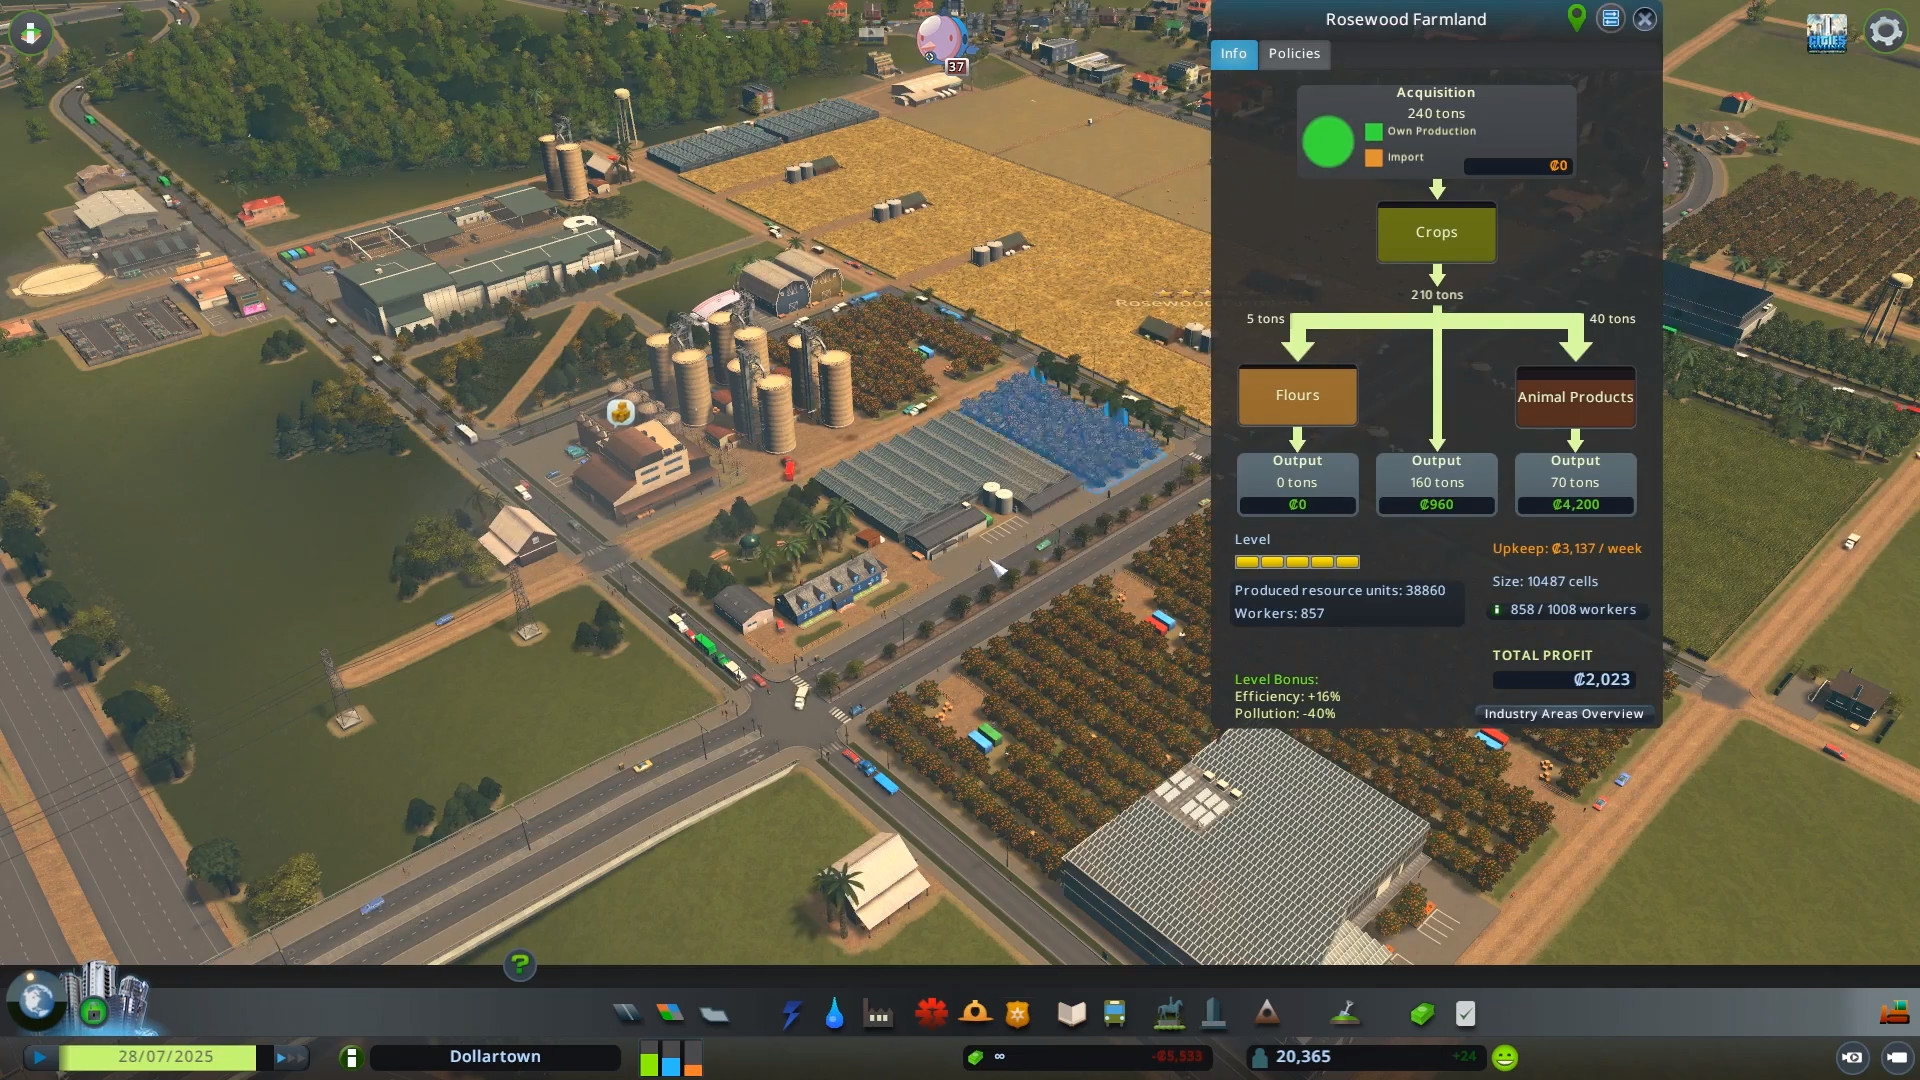
\includegraphics[width=\textwidth]{images/industries}
	\caption{Interfaz de gestión de recursos de la expansión \textit{Industries}}
	\label{fig:industry}
\end{figure}

Además, desde la expansión de \textit{Sunset Harbor} existe la industria pesquera, que agrega como recurso natural el pescado. Siguiendo el sistema de producción agregado en \textit{Industries}, este se puede procesar hasta obtener productos de consumo que se puedan exportar o vender en comercios. Dependiendo de la profundidad y el flujo del agua, se generará uno de los cuatro tipos de pescados: anchoas, atún, salmón y marisco. La polución en el agua provoca que desaparezcan este recurso del agua.

\section{Proceso de ingeniería}

En este capítulo se explica el proceso que se ha seguido para realizar el proyecto descrito. Se empezará explicando la metodología de desarrollo escogida y a continuación se expondrá y se desgranará la gestión de este trabajo.

\subsection{Metodología de desarrollo}
\label{subsec:metodologia}

A pesar de que en un primer se ha pensado que para la planificación de este proyecto se usaría la metodología de desarrollo SCRUM\cite{Schwaber:2001:ASD:559553}\cite{Schwaber:2004:APM:984028}, finalmente se ha optado por usar una amalgama entre distintas metodologías de desarrollo en espiral. Esto es debido a que SCRUM tiene unas características básicas que no se han tenido en cuenta a la hora de diseñar y desarrollar el proyecto, por lo que no sería correcto decir que se ha utilizado este tipo de metodología ágil:

\begin{itemize}
	\item \textbf{Flujo de trabajo}: El trabajo se divide en varias iteraciones entre una y cuatro semanas llamadas \textit{Sprint}, en donde en cada una de ellas se obtiene un incremento funcional del producto. Al comienzo de cada iteración se realiza una reunión en donde se identifican las tareas a realizar en esa iteración, realizando una estimación de todas; durante la realización de la iteración se realiza cada día una pequeña reunión en donde se comunica el estado actual; y, al finalizar una iteración se realiza una reunión que sirve como retrospectiva y alimentación para la próxima iteración.
	
	A la hora de realizar este proyecto, a pesar de que se ha dividido en varias iteraciones, realizando una reunión al principio de estos, y en cada iteración se finaliza con un producto funcional, el resto de elementos de la metodología SCRUM no se han llevado a cabo en la práctica.
	
	\item \textbf{Gestión de riesgos}: Uno de lo puntos de desarrollo con una metodología ágil es la de mantener una gestión de temprana de riesgos para evitar una gran desviación de la planificación. Esto se realiza mediante un panel que presenta listado ordenado de las tareas a realizar en el desarrollo total del proyecto, llamado \textit{Product backlog}. Estas tareas son las que estiman su duración y se incluyen en otro listado de tareas a realizar en cada iteración, llamado \textit{Sprint backlog}. Con esto se puede obtener una gráfica de evolución del proyecto llamado \textit{Burn down chart}, pudiendo detectar desviaciones y sobreasignaciones de forma visual debido a que también se marca el trabajo ideal de proyecto.
	
	Para este proyecto no se ha usado ninguno de estos elementos porque no se ha realizado un seguimiento exhaustivo del mismo a causa de la escasa experiencia de alumno a la hora de realizar una planificación y estimación del proyecto, sobre todo a la hora de seguir y diseñar un proyecto con una metodología de desarrollo ágil.
\end{itemize}

Debido a todos estos factores expuestos, se podría indicar que la metodología usada finalmente está más cerca de una basada en modelos de prototipos en donde se tiene en cuenta que cada prototipo resultante de una iteración es un modelo funcional del mismo, y en donde es revisado en la reunión de la siguiente iteración sin estar presente el cliente final, si no que solo con el director del proyecto. También en esta reunión se definen las tareas a realizar para el desarrollo del proyecto de cara a la nueva iteración.

\subsection{Gestión del proyecto}
\label{subsec:gestion}

A continuación se describirá la planificación llevada a cabo para cumplir con el tiempo estimado de realización del proyecto, así como el coste y los recursos necesarios para la construcción del mismo.

\subsubsection{Planificación}

TODO...

\subsubsection{Coste y recursos}

TODO...

\section{Análisis del software}

Una vez definido el sistema y planificada su construcción, se ha realizado un análisis en donde se identifican los requisitos que debe cumplir el software una vez terminado el proyecto.

\subsection{Requisitos funcionales}
\label{subsec:funcrequirements}

Los requisitos funcionales son aquellas condiciones indispensables que estipulan las funcionalidades que debe proporcional el sistema. Para este proyecto se ha recogido los diferentes requisitos:

\begin{itemize}
	\item Generación de un poligono industrial que sea legible por el videojuego \textit{Cities: Skylines\textcopyright}.
	\item Permitir añadir restricciones sobre ciertas zonas del mapa.
	\item Poder mostrar los resultados de la generación dentro del videojuego.
\end{itemize}

\subsection{Requisitos no funcionales}

Los requisitos no funcionales, por su contra, son aquellas condiciones indispensables que debe cumplir el sistema a la hora de diseñar e implementar. Para este proyecto se han tenido en cuenta estos requisitos:

\begin{itemize}
	\item Eficiencia y eficacia: El generador debe responder en el menor tiempo posible arrojando una respuesta óptima.
	\item Escalabilidad: El generador debe trabajar con mapas de diferentes tamaños, por lo que el sistema debe poder soportar cualquier tamaño de entrada.
	\item Usabilidad: La interfaz gráfica debe ser lo más sencilla posible, evitando que el usuario tenga que realizar tareas tediosas a la hora de construir mapas.
\end{itemize}

\section{Diseño del sistema}

Una vez definidos los requisitos se ha procedido a realizar el diseño software del sistema en cuestión, empezando a concretar la arquitectura propuesta y luego desarrollando los casos de uso y diagramas de clases.

\subsection{Arquitectura software}
\label{subsec:arquitectura}

Este proyecto se ha dividido en dos componentes concretos, que cada uno realiza una funcionalidad distinta. Esto es debido a que las tecnologías que usa \textit{Cities: Skylines\textcopyright} y \textit{Clingo} son distintas. Para ello se ha hecho un wrapper de la API C de \textit{Clingo} (llamado Clingo\# o ClingoSharp) para poder usarla en proyectos en C\#, y un mod que implementa las interfaces de \textit{Cities: Skylines\textcopyright} (IndustryLP) y que sirve como conexión entre el juego y la herramienta de \textit{Answer Set Programming}. La arquitectura del sistema se resume en la Figura \ref{fig:arquitectura}. \\

\begin{figure}[!h]
	\centering
	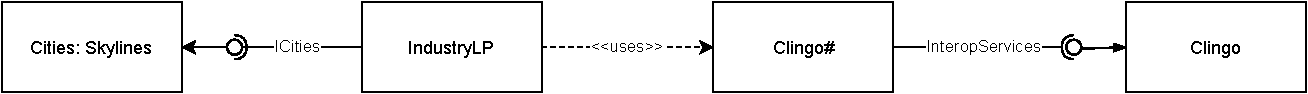
\includegraphics[width=\textwidth]{images/arquitectura.pdf}
	\caption{Arquitectura del sistema.}
	\label{fig:arquitectura}
\end{figure}

Cabe destacar que ClingoSharp se ejecuta en paralelo a IndustryLP, pudiendo este último enviar mensajes a ClingoSharp sin causar que la interfaz se congele, ademas de servir como recolector de errores que se puedan originar en nuestro programa lógico. Además, debido a que ClingoSharp funciona como wrapper de la API C de \textit{Clingo}, prevenimos la propagación de errores en el caso de que cambiase la API C de \textit{Clingo}, teniendo que cambiar solamente el componente ClingoSharp.NativeWrapper, tal y como se muestra en la Figura \ref{fig:clingosharp}. \\

\begin{figure}[!h]
	\centering
	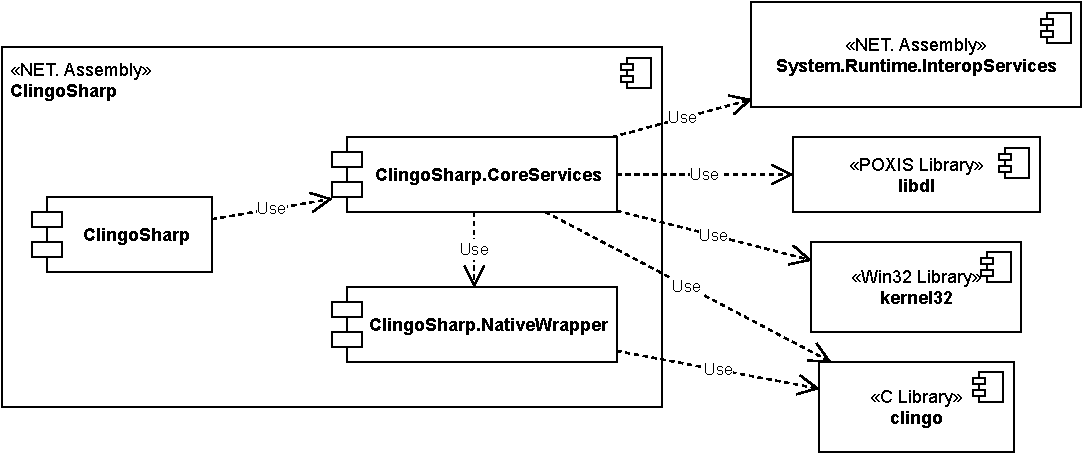
\includegraphics[width=\textwidth]{images/clingosharp.pdf}
	\caption{Arquitectura de ClingoSharp.}
	\label{fig:clingosharp}
\end{figure}\textbf{}

\subsection{Casos de uso}
\label{subsec:cases}

TODO

\subsection{Pantallas del sistema}
\label{subsec:mockups}

TODO

\subsection{Diseño del programa lógico}
\label{subsubsec:generator}

Retornando a lo comentado en la Sección \ref{subsec:arquitectura}, una de las piezas fundamentales de este proyecto es la definición de un generador de póligonos industriales en formato declarativo. Este módulo está pensado mediante el paradigma de programación lógica que usa \textit{Answer Set Programming}, tal y como se expone en la Sección \ref{subsec:asp}. Con esto el objetivo de este generador es intentar dar un modelo declarativo basado en reglas que corresponda en mayor o menor medida con la definición de un polígono industrial. \\

\subsubsection{Generación de edificios}

\begin{lstlisting}[label=lst:def]
	asp code
\end{lstlisting}

TODO

\subsection{Implementación}
\label{subsec:implementacion}

TODO